%!TEX root = ../report.tex

\chapter{Solution}


In this project, a system was implemented which is able to the record human demonstrations as kinematic trajectories, learn the motion in the form of dynamic motion primitive, reproduce the motion using dynamic motion primitives and execute this motion with mobile manipulator. This chapter discusses the actual design and the implementation of the software system. 

\section{Software Components}

Fig. \ref{fig:framework} shows the architecture of the implemented software system. Let's discuss components of this architecture one-by-one.  

\subsection{demonstrated\_trajectory\_recorder}


 
\textit{demonstrated\_trajectory\_recorder} records the trajectory demonstrated by the teacher with the help of arUco marker board, in the Cartesian space. Recorded trajectory is stored in a $n\text{x}6$ matrix. This matrix is then stored on the disk in \textit{yaml} file. Although all 6 degrees of freedom (3 linear and 3 rotational) are recorded during the demonstration, only linear degrees of freedom (X,Y,Z) are used for learning as demonstration of rotational degrees of freedom using arUco marker is difficult. Once the trajectory is recorded, it is also published on a \textit{rostopic} as a \textit{naviagation path} message for visualization in \textit{rviz}. 

\subsection{ros\_dmp} \textit{ros\_dmp} module consists of core DMP framework implementation called \textit{pydmps}, which is taken from internet source \cite{pydmps}. Implementing core DMP framework is fairly simple and straight forward, hence instead of implementing it from scratch, efforts were focused towards adapting already available implementation for Robot Operating System and robots. Changes were made in the original package so that it can be integrated with Robot Operating System and can be used on the robot. Changes include:
\begin{itemize}
	\item Addition of a method for retrieval of the weights of learned DMP.
	\item Modification in \textit{roll()} method to allow passing already learned weights.
	\item Removing unnecessary code for visualization. 
	\item Transforming package into a \textit{catkin} package so that it can be used as library in ROS workspace.
\end{itemize} 

Module \textit{learn\_motion\_primitive} provides the interface for learning the motion primitives from recorded trajectories. It reads recorded trajectory stored in \textit{yaml} file, uses the functionalities provided by the package \textit{pydmps} to learn motion primitive, stores weights in the another \textit{yaml} file and visualizes the learned DMP using \textit{RVIZ} tool in ROS.

Module \textit{roll\_dmp} reads the weight file associated with desired DMP to be executed. It takes the target end-effector pose in Cartesian co-ordinates as goal input and generates trajectory using functionalities provided by \textit{pydmps} package. It is also possible to solve the \textit{transformation system} step by step at fixed time intervals to generate instantaneous motion commands. This is necessary in the scenario where feedback from the environment and robot is needed to be incorporated in the DMP. One example of such feedback is on-line goal modification.      



\begin{figure}[H]
	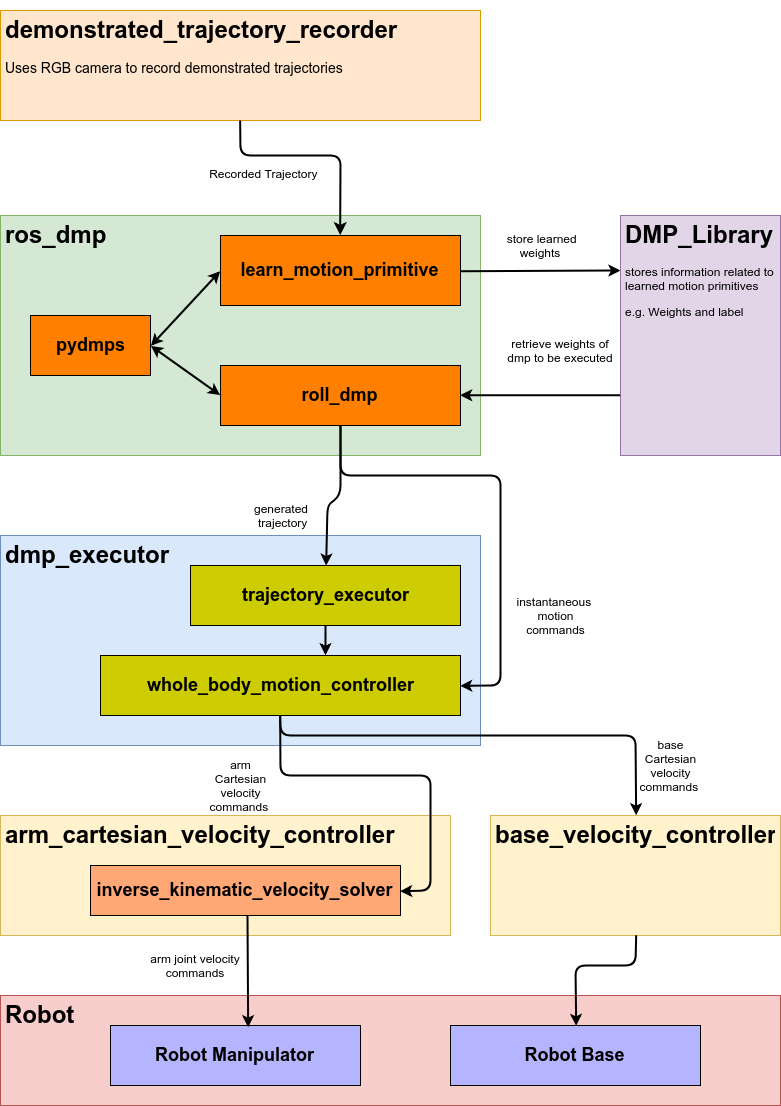
\includegraphics[width=\textwidth]{images/framework.png}
	\caption{Learning from Demonstration framework}
	\label{fig:framework}
\end{figure}


\subsection{DMP\_Library} \textit{DMP\_Library} is a collection of \textit{yaml} files containing learned weights of DMPs. Files are labeled appropriately so that the weights can be retrieved whenever necessary.



\subsection{dmp\_executor}

\textit{dmp\_executor} acts as the upper level control unit which executes trajectories or motion commands generated by \textit{roll\_dmp} module in \textit{ros\_dmp} package. \textit{trajectory\_executor} receives desired trajectory from \textit{ros\_dmp} and passes the velocity command to \textit{whole\_body\_motion\_control} unit, at each time step. Instead of using time as a velocity update parameter, it takes feedback of the pose of the end-effector and applies appropriate velocity command when end-effector reaches at particular position on the path.  


\textit{whole\_body\_motion\_control} receives the velocity command from \textit{trajectory\_executor} or directly from \textit{roll\_dmp} module. The velocity command is then processed according to the policy described in section \ref{whole_body_motion} to obtain end-effector velocity and base velocity. These velocities are then passed to respective low level controllers.

\subsection{arm\_cartesian\_velocity\_controller}

This package is a upgraded version of the package \textit{mcr\_arm\_cartesian\_control} in \textit{mas\_common\_robotics} library of b-it-bots. This package use \textit{OROCOS KDL (Kinematics and Dynamics Library)} library for calculating joint velocities for required Cartesian velocities of the end-effector frame. Class KDL::ChainIkSolverVel\_wdls in \textit{OROCOS KDL} implements the method described in section \ref{IK}. 

To use the previously implemented package in this project, some crucial changes were needed in order to meet new requirements. These requirements are:

\begin{itemize}
	\item Accessing singular values of Jacobian of the manipulator. (refer section \ref{IK} for singular values) 
	\item A way to change task space weights used in method described in \ref{IK}.
	\item Compatibility with new Toyota HSR robot. 
\end{itemize} 

Real time access to the singular values is necessary for calculating velocity commands for whole body motion control. Old package \textit{mcr\_arm\_cartesian\_control} uses old version of KDL which is the default version of KDL in ROS Kinetic. This version of KDL does not provide interface to access singular values in real time. Hence the old package is adopted for new version of KDL. A method was created to publish singular values on a \textit{rostopic} in real time. 

As both of the manipulators used in the experiments have 5 degrees of freedom, it is necessary to update task-space weights used to loosen the constraints on relatively less important motions in specific degree of freedom in real time. Hence a function was implemented which listen to a \textit{rostopic} on which weights can be published. This function updates the weights upon receiving new weights.   

Velocity message types used in Toyota HSR robot are different than those being used in KUKA YouBot, hence it was necessary to upgrade old package to use message types that can be used by both robots.         

\subsection{Robot}

Once the joint velocity commands and the linear velocities for the base are generated, they are published on respective \textit{rostopics}. These \textit{rostopics} are subscribed by the respective hardware interface components, which are responsible for the execution of motion commands. Study and analysis of these components is out of the scope of this project.  



